%!TEX encoding = IsoLatin
\documentclass[conference]{IEEEtran}

\usepackage{cite}
\usepackage{graphicx}
\usepackage{amsmath}
\usepackage{algorithmic}
\usepackage{fixltx2e}
\usepackage{stfloats}
\usepackage{url}
\usepackage{hyperref}
\usepackage[latin1]{inputenc}
\usepackage{lipsum}
\usepackage{coolMath}
\usepackage[hang,small]{caption}
\graphicspath{{Images/}}

\title{Relevance Vector Machine for regression and comparaison with the SVR}
\author{
	\IEEEauthorblockN{Hadrien Hendrikx}
	\IEEEauthorblockA{
					School of Engineering (STI)\\
					\'Ecole Polytechnique \\ F�d�rale de Lausanne\\
					Lausanne, Switzerland\\
					hadrien.hendrix@epfl.ch
					}\\
	\and
	\IEEEauthorblockN{Gregoire Gallois-Montbrun}
	\IEEEauthorblockA{
					School of Engineering (STI)\\
					\'Ecole Polytechnique \\ F�d�rale de Lausanne\\
					Lausanne, Switzerland\\
					gregoire.gallois-montbrun@epfl.ch
					}
	\and
	\IEEEauthorblockN{Louis Faury}
	\IEEEauthorblockA{
					School of Engineering (STI)\\
					\'Ecole Polytechnique \\ F�d�rale de Lausanne\\
					Lausanne, Switzerland\\
					louis.faury@epfl.ch
					}
	}
	
\begin{document}

	\maketitle
	
	\begin{abstract}
		This report, written in the context of a machine learning coding project, compares two sparse regression techniques. \newline After introducing some theoretical aspects on Support Vector Regression (SVR) and the Relevance Vector Regression (RVR), we introduce two datasets (an artificial one as well as a real one) that will serve us as baselines for experimental comparisons between the two methods. 
		\newline We will then focus the comparison on a few key features. Namely, we will study the tradeoff found between generalization and sparsity in the two methods. Issues such as robustness (behavior far from data, dataset scavenging and data chunking), computational complexity and training / testing time will also be tackled. 
	\end{abstract}
	
	\section{Introduction}
	{
		We hereinafter focus on regression tasks : from a dataset $\{X,\mathbf{t}\} \in\mathbb{R}^{N,d}\times\mathbb{R}^N$, we wish to learn a function $f$ such that $f(X)\simeq \mathbf{t}$. 
		\newline The simplest method to perform such a task is to consider that $f(\cdot)$ is a linear function of a non-linear mapping of the input $x$, corrupted by a normally distributed noise of precision  $\beta$ 
		\begin{equation}
			t = w^T\phi(x) + \eta, \quad \eta \sim \normalDb{\eta}{0}{\beta^{-1}} 
		\end{equation} 
		with $\phi\, : \, \mathbb{R}^d \to \mathbb{R}^m$ a non-linear transformation. 
		Therefore, $p(t\, \vert \, w,\beta)\sim \normalDb{t}{w^T\phi(x)}{\beta^{-1}}$ and the \emph{maximum-likelihood} solution is given by the minimizer of the opposite of the log-likelihood : 
		\begin{equation}
			w_{MLE} = \argmin{w}{\frac{1}{2}\sum_{n=1}^N\left\{w^T\phi(x_n) - t_n\right\}^2}
		\end{equation}
		To avoid overfitting, a regularizer term is often added to the cost function :
			\begin{equation} 
							E(w) = \frac{1}{2}\sum_{n=1}^N\left\{w^T\phi(x_n) - t_n\right\}^2 + \frac{\lambda}{2}\lVert w \rVert ^2
							\label{eq::ridge}
			\end{equation}
		even if some more advanced methods (Bayesian learning for instance) can also be used to avoid prevent data overfit. 
	}
	\section{Theoretical background}
	{
		\subsection{Support Vector machine for Regression}
		{
			The Support Vector machine for Regression (SVR) extends the SVM method for regression tasks.
			\newline
			To obtain a sparse solution, the likelihood term in (\ref{eq::ridge}) is replaced by an $\eps$-\emph{insensitive error function} (see \cite{vapnik1995nature}) denoted $E_\eps(\cdot)$ with : 
			\begin{equation}
				\label{eq::loss}
				E_\eps(y(x)-t) = \left\{
								\begin{aligned}
								&0, \quad &\text{ if } \vert y(x)-t\vert < \eps\\
								& \vert y(x)-t\vert < \eps \quad &\text{otherwise}  
								\end{aligned}\right.
			\end{equation}
			Therefore, the quantity to be minimized can be expressed as : 
			\begin{equation}
				J(w) = \frac{C}{n}\sum_{n=1}^N E_\eps(w^T\phi(x_n)-t_n) + \frac{1}{2}\lVert w \rVert ^2
			\end{equation}
			where $C$ is a regularization parameter. 
			\newline 
			As for the SVM, one can introduce \emph{slack variables} in order to transform this optimization program into a Quadratic Programming (QP) problem (quadratic objective, linear constraints) : 
			
			\begin{mini}|s|[2]
  				 {w,b}{\frac{1}{2}\lVert w \rVert^2 + \frac{C}{n}\sum_{i=1}^n{\left(\xi_i + \hat{\xi}_i\right)}}
  				 {\label{eq::svr}}{}
   				\addConstraint{\xi, \hat{\xi}}{\geq 0}{\text{ (row wise) }}
  				 \addConstraint{w^T\phi(x_i)+b + \eps + \xi_i  }{\geq t_i,\quad}{i=1,\hdots,n}
				\addConstraint{w^T\phi(x_i)+b - \eps - \hat{\xi}_i  }{\leq t_i,\quad}{i=1,\hdots,n}
			\end{mini}
				
			Once the problem solved, predictions are made using : 
			\begin{equation}
				y(x) = \sum_{n=1}^N (a_n - \hat{a}_n)k(x,x_n) + b
			\end{equation}
			where we introduced the kernel $k(x,x') = \phi(x)^T\phi(x')$. The coefficients $\{a_n\}$ and $\{\hat{a}_n\}$ actually are Lagrange multipliers for the QP problem (\ref{eq::svr}), and provide a \emph{sparse} solution  - only a few data points are used for regression. Those are called \emph{support vectors}, and are so that  $a_n \neq 0$ or $\hat{a}_n\neq 0$ - in other words, those that lie on the boundary or outside of the $\eps$-tube defined by the loss function in equation (\ref{eq::loss}). \newline
			As for the SVM, one can adopt a $\nu$-SVR formulation (see \cite{scholkopf2000new}) to have a \emph{lower-bound control} on the number of retained support vectors. 
		}
		\subsection{Relevance Vector machine for Regression}
		{
			The SVR therefore provides a useful tool for obtaining sparse regression machine. However, it suffers from a \emph{number of limitations}, such as an output representation as decision rather than posterior probability, the need to estimate hyper-parameters (kernel width, penalization parameter) via \emph{held-out methods} (like cross-validation), or the need for the kernel to be a Mercer kernel type (positive definite). 
			\newline
			The Relevance Vector Machine for regression is a \emph{Bayesian sparse kernel technique} that shares many of the SVR's characteristics while avoiding its limitations. It instantiates a model intended to mirror the structure of the SVR : 
			\begin{equation}
				y(x) = \sum_{n=1}^{N+1}w_nk(x,x_n)
			\end{equation}
			where the bias $b$ is included in the predictor $w$ and $k(\cdot,\cdot)$ is an arbitrary kernel (not necessarily positive definite). Assuming i.i.d data sample with Gaussian noise of precision $\beta$, the likelihood writes : 
			\begin{equation}
				\condp{\mathbf{t}}{X,w,\beta} = \prod_{n=1}^N \normalDb{t_n}{y(x_n)}{\beta}
			\end{equation}
			The predictor $w$ is given a centered Gaussian prior distribution :
			\begin{equation}
				\condp{w}{\alpha} = \prod_{i=1}^{N+1} \normalDb{w}{0}{\alpha_i^{-1}}
			\end{equation}
			introducing a separate precision parameter $\alpha_i$ for each weight parameter $w_i$. 
			\newline 
			This leads to a Gaussian posterior distribution over $w$ : 
			\begin{equation}
				\begin{aligned}
					\condp{w}{\mathbf{t},X,\alpha,\beta} &= \condp{\mathbf{t}}{w,X,\beta}\condp{w}{\alpha}\\
												&= \normalDb{w}{m}{\Sigma}
				\end{aligned}
			\end{equation}
			where 
			\begin{equation}
				\begin{aligned}
					m &= \beta \Sigma \boldsymbol{\phi}^T t\\
					\Sigma &= \left(A+\beta \boldsymbol{\phi}^T\boldsymbol{\phi}\right)^{-1}, \qquad A = \text{diag}(\alpha_i)
				\end{aligned}
				\label{eq::posterior}
			\end{equation}
			In a full Bayesian approach, $\alpha$ and $\beta$ are both given prior distributions. However, this leads to intractable computations when computing predictions. The use of \emph{empirical Bayes} solves this problem, by approximating $\alpha$ and $\beta$ by their maximum-a-posteriori value (also known as the \emph{evidence approximation} or type-2 maximum likelihood). \newline
			As a result of approximation, a proportion of parameters $\alpha_i$ are driven to infinite values, constraining the corresponding weights $w_i$ to have $0$ mean and infinite precision, and hence are set to $0$. The resulting predictions are therefore sparse in data-points, and the inputs $\{x_n\}$ corresponding to non-zero weights are called \emph{relevance vectors}. Once the optimal values $\alpha^*$ and $\beta^*$ found, the predictive distribution over $y$ can therefore be computed using $\alpha^*$ and $\beta^*$. 
			\newline The sparsity analysis of the RVR leads to a practical algorithm for optimizing the hyper-parameters that has significant speed advantages, and is referred to as \emph{automatic relevance determination}. The full algorithm and its justification can be found in \cite{bishop2006pattern} and \cite{tipping2003relevance}.
			\newline Furthermore, the RVR provides a posterior distribution over the predictor, leading to the following \emph{predictive distribution} (unlike the SVR which only provide a posterior decision) : 
			\begin{equation}
				\begin{aligned}
					\condp{t}{x,X,\mathbf{t},\alpha,\beta} &= \int_w \condp{t}{w,x,\beta}\condp{w}{X,\mathbf{t},\alpha}dw\\
					&= \normalDb{t}{m^T\phi(x)}{\phi(x)^T\Sigma \phi(x)}
				\end{aligned}
				\label{eq::predictive}
			\end{equation}
			with $m$ and $\Sigma$ the first moments of the posterior (see (\ref{eq::posterior}))
		}
		\subsection{Theoretical method comparaison}
		{
			\subsubsection{Complexity}
			{
				When comparing the SVR's and the RVR's complexity, one must distinguish complexity at training time and at testing time. \newline
				Training the SVR sums up in solving a large quadratic-programing (QP) problem. A popular approach to do that implies breaking up the initial QP into smaller problems, solvable analytically, and is called \emph{Sequential Minimization Optimization} (SMO). It requires a linear (with respect to the datapoints) amount of memory, and scales between linear and quadratic complexity in the training set size (see \cite{platt1998sequential}). At test time, the complexity is linear in the number of support vectors. \newline
				Training a RVM involves optimizing a non-convex function. For a model with $M$ basis functions, the RVM requires the inversion of a $M\times M$ matrix, which requires from $O(M^{2.7})$ to $O(M^{3})$, which is as we just saw larger than the SVR's cost. However, parameters are determined automatically and in one run when training a RVR, while the hyper-parameters typically need several runs (f-fold cross-validation) to be estimated. At testing time, the RVR's complexity grows linearly with the number of relevance vectors.  
			}
			\subsubsection{Performance}
			{
				We just named one of the major pros of using RVR - there is no need for using held-out methods to estimate hyper-parameters, as they are automatically determined through automatic relevance detection (expect for parametric basis functions). Also, it has been shown \cite{platt1998sequential, bishop2006pattern} that RVR leads to \emph{sparser solutions, without loss of generalization abilities} (on the contrary, the RVR usually performs better than the SVR). We will try to observe this observations in the experiments derived hereinafter.
			}
		}
	}
	\section{Results}
	{
		\subsection{Datasets presentation}
		{
			\subsubsection{Artificial dataset}
			{
				The goal of using an artificial dataset is to be able to produce visual outputs to evaluate the performance of the two methods on a simple regression problem, hence the need to work in a one dimensional dataset. 
				\newline The dataset was generated from the $sinc(\cdot)$ function, on the interval $[-5,5]$. Points were randomly sampled from this interval, applied the $sinc$ function and added a normally distributed noise. For reasons we'll tackle later, no outliers were added in the dataset.
				\newline The following table sums up the dataset characteristics. 
				\vspace{3pt}
				
				\noindent\begin{tabular}{|c|c|c|c|c|}
				\hline 
					\textbf{Dimension} & \textbf{Points} & \textbf{Support} & \textbf{Noise variance} & \textbf{Outlier} \\
					\hline
					1 & 100 & [-5,5] & 0.01 & No\\
					\hline
				\end{tabular}
				
				\begin{figure}[h!]
					\centering
					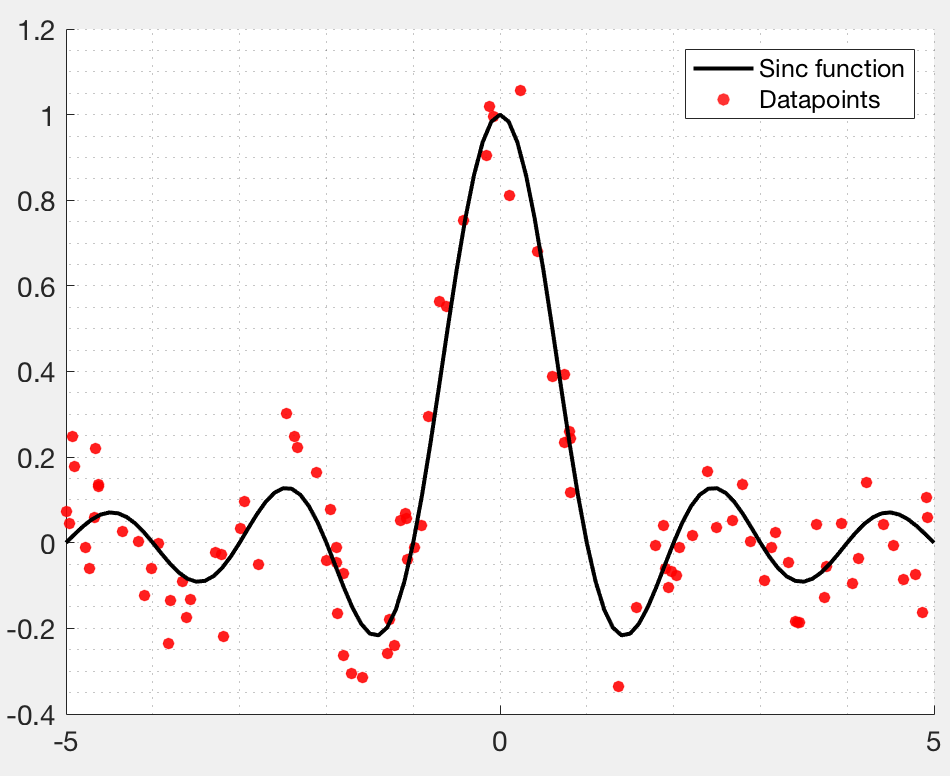
\includegraphics[width=0.6\linewidth]{dataset_1d}
					\caption{The 1D artificial dataset}
				\end{figure}
			}
			\vspace{5pt}
			
			\subsubsection{Real dataset}
			{
				%This dataset, known as the Online News Popularity dataset, provide informations about a web article (number of words, number of link to other articles, number of images or videos, ..) to predict its number of shares in social network (see \cite{fernandes2015proactive} for full details). The following table sums up the dataset characteristics. 
				
			        %\begin{center}
				%\noindent\begin{tabular}{|c|c|}
				%	\hline 
				%	\textbf{Dimension} & \textbf{Points} \\
				%	\hline
				%	58 & 30493\\
				%	\hline
				%\end{tabular}
				%\end{center}
				This dataset, known as the Airfoils Self-Noise dataset provides informations about design of various airfoils and physical environment (free stream velocity, angle of attack, chord length, frequency, suction side thickness) in order to predict the resulting sound pressure level in dB (see \cite{brooks1989} for full details). The following table sums up the dataset characteristics.
				
				\vspace{3pt}
				
				\begin{center}
				\noindent\begin{tabular}{|c|c|}
					\hline 
					\textbf{Dimension} & \textbf{Points} \\
					\hline
					5 & 1503\\
					\hline
				\end{tabular}
				\end{center}	
			}
		}
		\subsection{}
		{
			We hereinafter describe different computations and results obtained on the artificial data with both the SVR and the RVR. Discussion on the two methods advantages and drawback will be held in the next section.
			
			\subsubsection{Support Vector Regression}
			{
				We implemented both the $\eps$-SVR and the $\nu$-SVR on the artificial dataset. We used the \texttt{libsvm} library (see \cite{libsvm}) with a radial-basis function kernel : 
				\begin{equation}
					\forall x,x', \quad k(x,x') = \exp{\left( -\frac{\lVert x -x'\rVert^2}{\sigma^2}\right)}
				\end{equation}
				
				We therefore have to tune three hyper-parameters : $\sigma$ (kernel width), $C$ (penalization factor) and $\nu$ (resp. $\eps$) for the $\nu$-SVR (resp. $\eps$-SVR). Figures (\ref{nuSVR}) and (\ref{epsSVR}) display the regressive function obtained for three given parameters for both methods on the artificial dataset. For the $\nu$-SVR, the corresponding $\eps$-insensitive tube was computed thanks to the values of the final Lagrange multipliers (a Lagrange multiplier strictly inferior to $C$ indicates a point laying on the $\eps$-tube). 
				\begin{figure}
					\begin{center}
						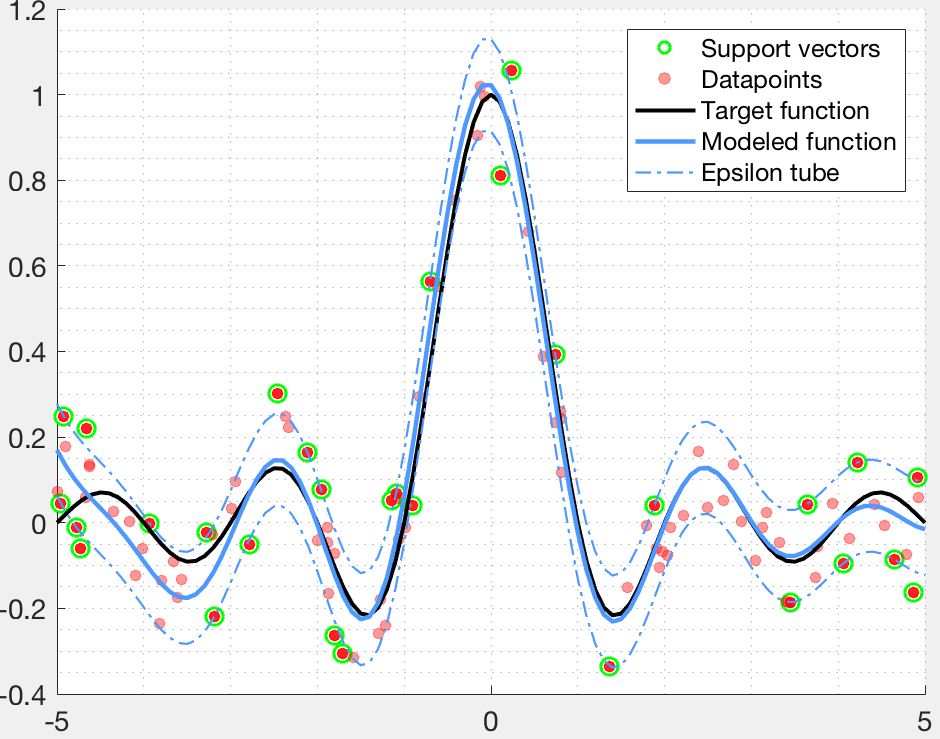
\includegraphics[width=0.85\linewidth]{nuSVR_nu02_C100_width02}
						\caption{$\nu$-SVR with : $C=100$, $\nu=0.2$, $\sigma = 1.5$}
						\label{nuSVR}
					\end{center}
				\end{figure}
				\begin{figure}				
					\begin{center}
						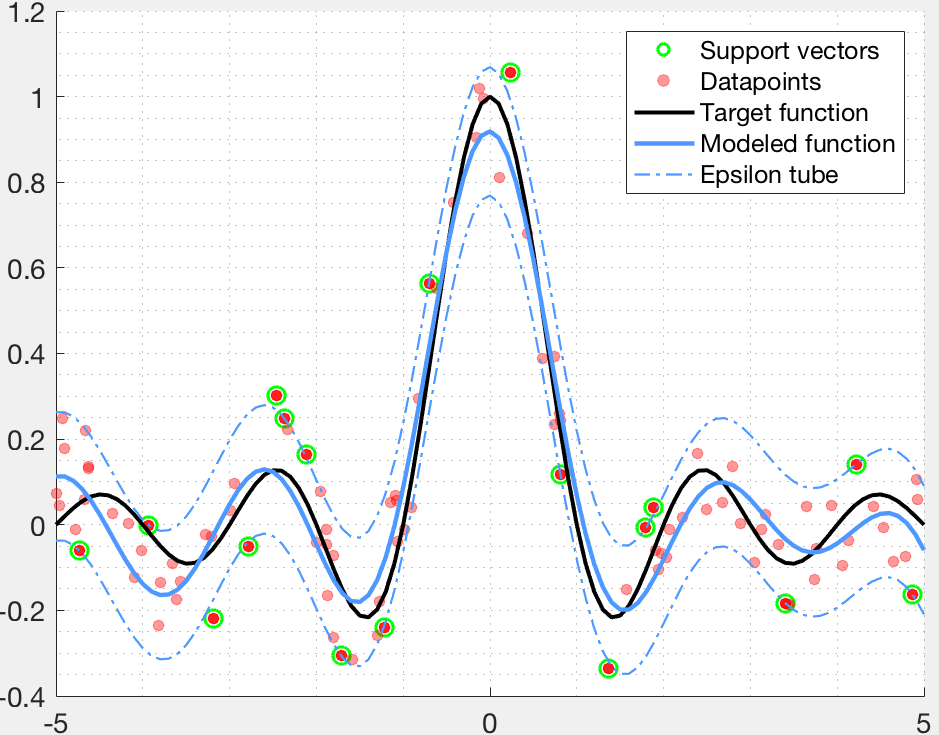
\includegraphics[width=0.85\linewidth]{epsSVR_eps015_C50_width2}
						\caption{$\eps$-SVR with : $C=50$, $\eps=0.15$, $\sigma = 2$}
						\label{epsSVR}
					\end{center}
				\end{figure}
			}
			\subsubsection{Relevance Vector Regression}
			{
				A similar work was conducted with the RVR. The same kernel (RBF) was used. Therefore, the only hyper-parameter to be fixed is the kernel's width $\sigma$ (since automatic relevance detection automatically finds the best $\beta$ and $\alpha$). For regression, we plot the mean of the \emph{predictive distribution} as well as it's standard deviation (see (\ref{eq::predictive})).
				
				\begin{figure}
					\begin{center}
						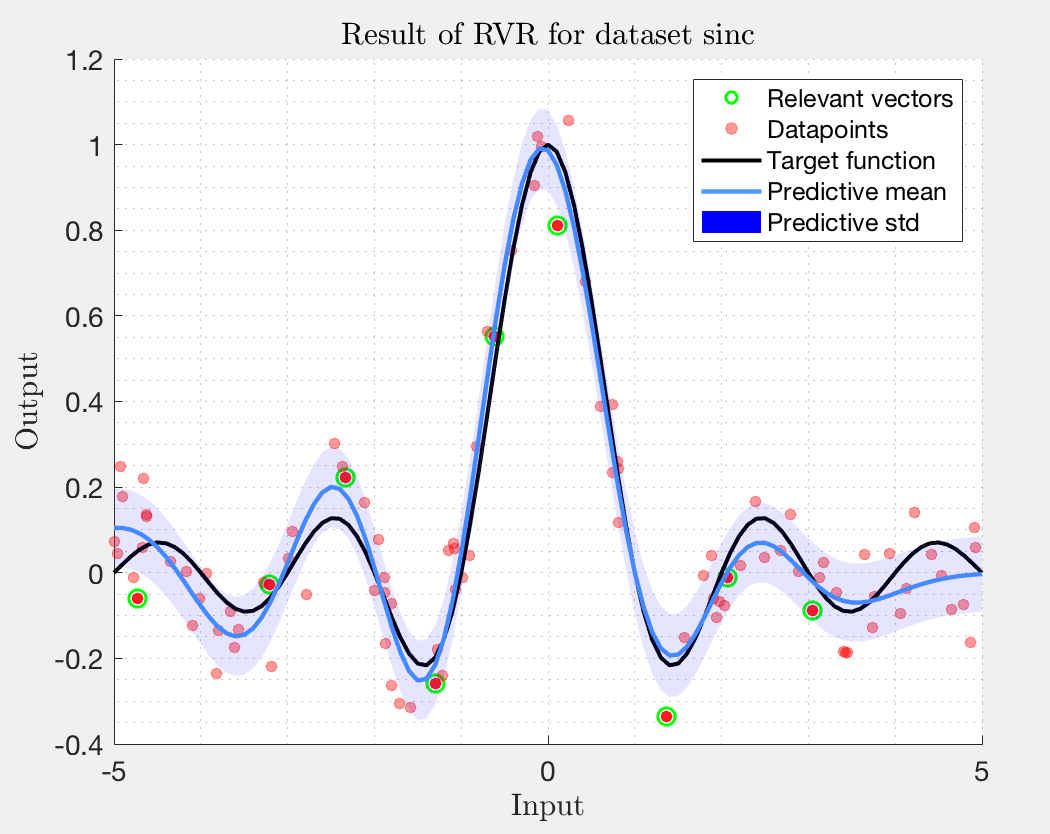
\includegraphics[width=0.85\linewidth]{RVR_width1}
						\caption{RVR with : $\sigma = 1$}
						\label{nuSVR}
					\end{center}
				\end{figure}
			}
		
		}
		\subsection{Cross-validation}
		{
			\subsubsection{Artificial dataset}
			{
			To assess best hyper-parameters for all three algorithms ($\epsilon$-SVR, $\nu$-SVR and RVR), grid search was performed using 50-fold cross validations. Training test ratio was set to 0.75. Chosen metric to evaluate performance of the algorithms is derived from the BIC (Bayesian Information Criterion). Among the properties of such metric is the ability to evaluate a compromise between complexity and likelihood of the different models. Compared to a metric like Mean Square Error, it therefore tends to favor model sparsity which is one of the main advantages of studied regression algorithms.
			
			General formula for BIC is:
			\begin{equation}
				BIC = -2ln(L) + kln(N)
			\end{equation}
			where $L$ corresponds to the likelihood of the model, $k$ is the number of parameters of the model and $N$ is the number of datapoints. In the case of RVR and SVR, number of parameters $k$ is directly proportional to the number  of relevant vectors and respectively support vectors. In both cases we relate likelihood of models to the Mean Square Error (MSE) as such:
			\begin{equation}
				ln(L) = -\frac{N}{2\sigma^2_{noise}}MSE
			\end{equation}
			where $\sigma^2_{noise}$ corresponds to the variance of dataset noise.
			
			For SVR, number of model parameters corresponds to the number of non-zero coefficients  $\alpha_i$ and $\alpha_i^*$. $k$ is therefore equals to twice the number of support vectors  ($N_{SV}$)so that:
			\begin{equation}
				BIC_{SVR} =  \frac{MSE}{\sigma^2_{noise}} + 2N_{SV}ln(M)
			\end{equation}
			
				\begin{figure}
					\begin{center}
						\includegraphics[width=0.85\linewidth]{gridsearch_epsSVR}
						\caption{Grid search for $\epsilon-SVR$ over $\epsilon$, $C$ and $\sigma$ for sinc dataset \\ Best hyperparameters: $\epsilon = 0.17$, $C = 2.40$, $\sigma = 1.17$}
						\label{fig::gridSearch_epsSVR_sinc}
					\end{center}
				\end{figure}
				
				\begin{figure}
					\begin{center}
						\includegraphics[width=0.85\linewidth]{gridsearch_nuSVR}
						\caption{Grid search for $\nu-SVR$ over $\nu$, $C$ and $\sigma$ for sinc dataset \\ Best hyperparameters: $\nu = 0.057$, $C = 1.52$, $\sigma = 1.13$}
						\label{fig::gridSearch_nuSVR_sinc}
					\end{center}
				\end{figure}
			
			Figures (\ref{fig::gridSearch_epsSVR_sinc}) and (\ref{fig::gridSearch_nuSVR_sinc}) display grid search results for both $\epsilon$-SVR and $\nu$-SVR in the form of a heat-map. As expected both selected models are almost the same therefore showing the equivalence between both approaches. Both lead to a total of 14 support vectors.\\
			
			For RVR, the number of free parameters $k$ corresponds to the non zero coefficients $w_i$ of the relevant vectors. It is therefore equals to $N_{RV}$, the number of relevant vectors. As a consequence, BIC for RVR writes:
			\begin{equation}
				BIC_{RVR} =  \frac{MSE}{\sigma^2_{noise}} + N_{RV}ln(M)
			\end{equation}
			
				\begin{figure}
					\begin{center}
						\includegraphics[width=0.75\linewidth]{gridsearch_RVR}
						\caption{Grid search for $RVR$  over $\sigma$ for sinc dataset. Best hyperparameter: $\sigma = 1.28$}
						\label{fig::gridSearch_RVR_sinc}
					\end{center}
				\end{figure}
			
			Figure (\ref{fig::gridSearch_RVR_sinc}) displays grid-search results over kernel width $\sigma$, the only hyperparameter.

			}
							
			\subsection{Real dataset}
			{
				For this dataset, the lack of information concerning dataset noise prevented to use BIC-like metrics for finding best hyperparameters. We therefore performed grid search using 10-fold cross validation over Mean Square Error for the different algorithms, after standardization of data. Such metric only considers fitting of the different models with the data without taking model complexity into account. Due to higher dimensionality and to an higher number of points, training test ratio was reduced to 0.5.
				
				Results of grid search over $\sigma$, the kernel width for Relevance Vectors Regression are displayed on figure (\ref{fig::gridSearch_RVR_airfoils}). Optimal kernel width therefore corresponds to $\sigma = 1.25$ leading to an MSE of 0.19. Number of retrieved relevance vectors is 94.
				
				\begin{figure}
					\begin{center}
						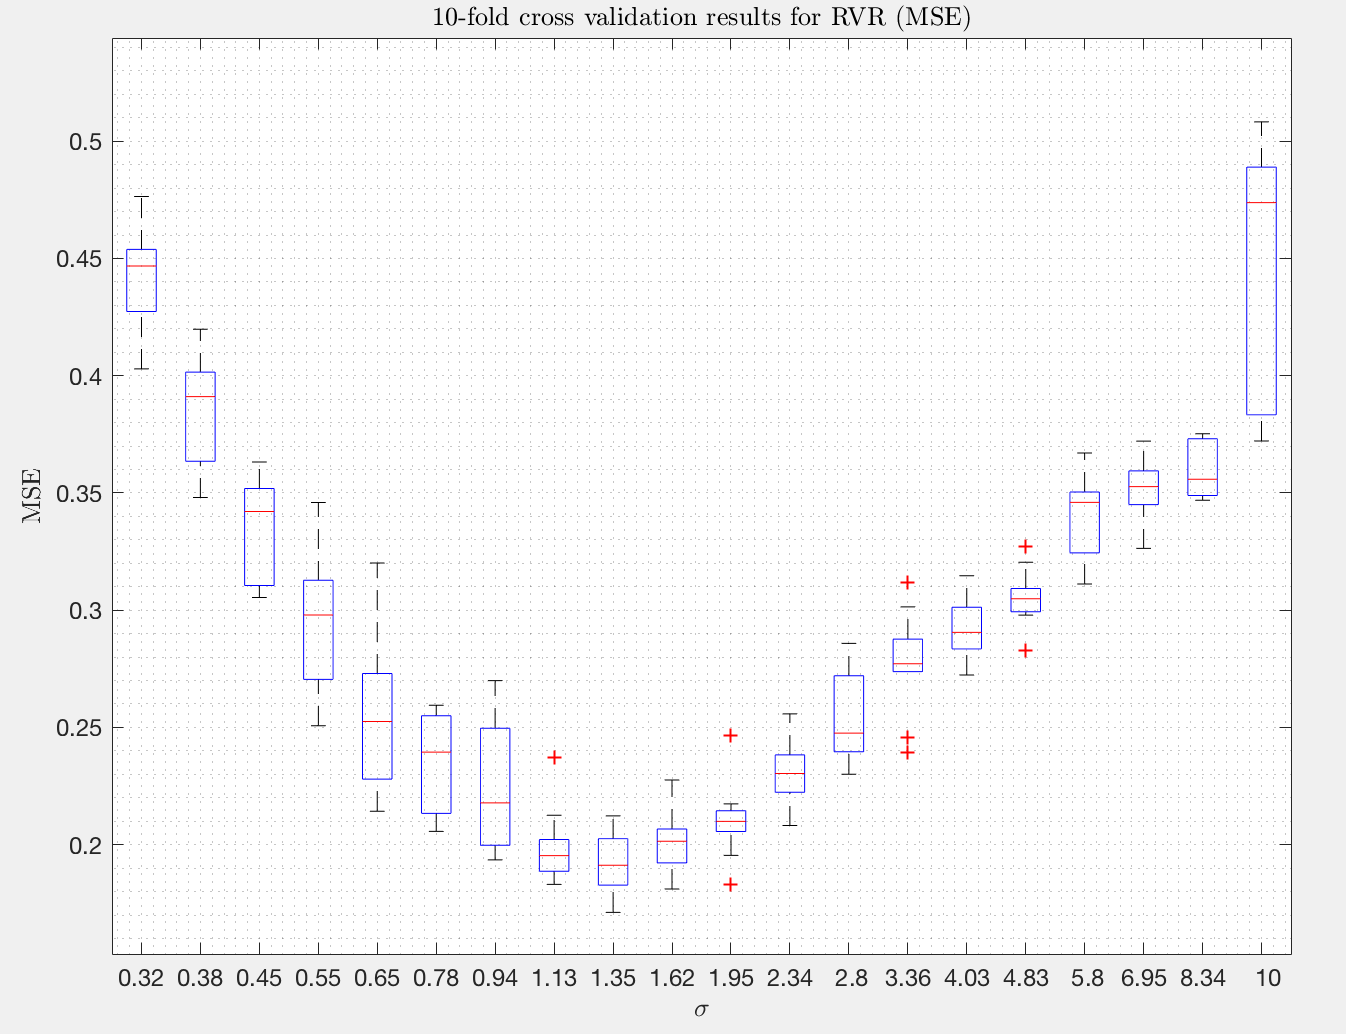
\includegraphics[width=0.8\linewidth]{airfoils_gridsearch_RVR}
						\caption{Grid search for $RVR$  over $\sigma$ for airfoils dataset. Best hyperparameter: $\sigma = 1.25$}
						\label{fig::gridSearch_RVR_airfoils}
					\end{center}
				\end{figure}
				
				
				
			}
			
		}
	}
	\section{Discussion}
	{

	}
	\section{Conclusion}
	{

	}
	
	\bibliographystyle{plain}
 	 \bibliography{bib_file}
	
\end{document}